% File: report.tex

\documentclass[letterpaper]{article}
\pdfoutput=1
\usepackage{aaai}
\usepackage{times}
\usepackage{helvet}
\usepackage{courier}
\usepackage[pdftex]{graphicx}
\usepackage{amssymb}
\frenchspacing
\pdfinfo{
/Title (Using A Hierarchical Architecture for Collaborative Social Tasks to Reinforce and Recognize Action Primitives)
/Subject (In Proceedings AAAI)
/Author (Bradley Hayes, Thaddeus Diamond, and Brian Scassellati)
}
  
\begin{document}
\title{Using A Hierarchical Architecture for Collaborative Social Tasks to Reinforce and Recognize Action Primitives}
\author{Bradley Hayes, Thaddeus Diamond, and Brian Scassellati\\
Yale University\\
Arthur K. Watson Hall\\
51 Prospect St\\
New Haven, Connecticut 06511\\
}

\maketitle

\begin{abstract}
 Recent work has shown that with human
assistance, complex actions can be learned with limited training data. The
resulting skill representations can be leveraged to replay flexible behaviors
that dramatically increase the utility of the robot. Despite this, existing
systems have yet to address the greater problem of cooperative action execution.
For a robot to effectively cooperate with either human or robotic coworkers,
the robot must be capable of modeling and recognizing its
coworkers' behaviors within its environment. We approach the task of
understanding and predicting coworker actions by providing a novel, fast algorithm
allowing a robot to solve skill recognition, the inverse problem of skill execution,
in real-time. Our algorithm provides a coded timeline of
primitive actions generated in real-time, correcting its hypotheses as more
information is presented. We demonstrate our results through the recognition of selected
American Sign Language gestures. Our work is unique in that it extends Q-Tables,
a product of Q-Learning that are consistently used to model skills,
to create a unified data structure capable of both skill execution
and skill recognition.  This data can then be directly used to facilitate the
creation of a skill hierarchy fully decomposing a complex cooperative 
task into primitive actions.
\end{abstract}

\section{Introduction}
\label{sec:intro}
% 1. Talk about the need for cooperative robotics here.
	As research in recent years has demonstrated, robots operating in a collaborative environment (co-robots) need to be flexible agents, adapting to the changing needs of their daily operations. An excellent example of such a system is Robonaut, a humanoid robot designed to match the dexterity of a suited astronaut \cite{Robonaut}. This platform is designed for both autonomous collaboration and teleoperative capabilities, a desirable set of operating modes for assisting human coworkers in the particularly challenging environment of outer space.
	
  The introduction of such systems requires a substantial effort not merely to produce capable and robust robots, but also to generate a careful and planned interaction method allowing non-expert human operators to contribute to the robot's training with a autonomous, intuitive procedure.  Observation is an extremely common method for teaching rudimentary skills required in a collaborative effort.  Therefore, it is important that a co-robot not only achieve competency through direct skill training, but also that it use observations of others in its everyday behaviors to reinforce and improve existing abilities.  For systems embodying these characteristics, maintaining an awareness of peer actions is critical for safety, efficiency, and general performance. Direct skill training is still, however, a vital part of a co-robot's success.  Knox et. al. \shortcite{TAMER2} continue to make progress towards allowing non-experts to guide skill acquisition in such systems, facilitating the design of agents with shapeable behaviors.
  
  We propose a novel method for online action classification that robotic agents can leverage to:
  \begin{itemize}
    \item Categorize a set of observed actions into labeled primitives and unknowns using Semi-Markov Decision Processes (SMDPs), the existing standard of skill representation in Q-Learning
    \item Help achieve this awareness while simultaneously using the observed data to improve its own performance and understanding of low level actions
    \item Facilitate the creation of a generic skill hierarchy fully decomposing a complex cooperative 
task into primitive actions
    \item Utilize the generated skill hierarchy in a generic hierarchical learning system in order to simultaneously execute primitive actions recognize known skills being performed by co-workers
  \end{itemize}

  We demonstrate our system's functionality by automating identification of selected American Sign Language gestures, while simultaneously using that observed data to improve our agent's internal representation of the underlying primitive skills involved. We then present the significance of this contribution, grounded within the rapidly expanding field of collaborative robotics.

\section{Background and Related Work}
\label{sec:background}
\subsection{Skill Recognition}
%1. Talk about LBD as an accessible means for non-experts to train robots on skills.
  Several methods have been proposed for automating skill acquisition in robots.  However, many of these have relied on using expert knowledge to transfer primitive actions of a specific domain to a system via programming.  Learning by demonstration (LBD), by contrast, is a technique that relies on prerecorded samples as a means for experts and non-experts alike to train robots on primitive actions.  The automation and accessibility of such methods have increased the complexity and variety of skills that a robotic system can successfully acquire.

%2. Introduce concept of learning skills through traditional robot QLearner system, talk about result: qtable and policy indicating possible executions of skill.
  How such a robotic system might represent primitive actions can vary.  Traditional robotic systems often use Markov Decision Processes in combination with Q-Learning to accomplish this goal.  The result of such an effort is both a \textit{Q-Table}, representing the known states in a given environment and the corresponding rewards for transitions between them, and a \textit{policy} indicating all possible executions of a skill.  Such a policy, in the simplest case, can be represented as a greedy traversal of the MDP until the goal state is reached.

%3. Introduce idea that this information can also be leveraged to identify others' execution of these skills
  Because a Q-Table can be viewed as an arbitrary n-dimensional representation of a given state space, it can be leveraged to identify the observed execution of known policies.  For example, assume a state space represents the positions of a right hand, right elbow, and right shoulder in three-dimensions.  A robotic system with a predefined dictionary of gestures could use standard statistical methods to decompose sensor data into timeframes labeled according to which of the robot's policies most closely matched during that interval.  In fact, that is exactly what our system does.

%5. Generalize result beyond gesture recognition to other motor tasks, cite konidaris' work
  It is important to note that gesture recognition is not the only domain in which our system is viable.  Several common motor tasks, such as tool manipulation and collaborative problem solving requiring an external perspective \cite{HRITraftonPerspective} are well-suited to utilizing a previously acquired set of action policies.

% 6. Present work as an enhancement layer for konidaris' CST work, generalizing it to automatically work for multiple skills, properly applying training data.
  The notion of using skill transfer is not entirely novel.  Konidaris et al. \shortcite{AutoSkillAcquisition} have successfully leveraged existing learned skills to perform manipulation of simple tools. However, our major contribution is that the skill transfer resides not in transferring knowledge across domains, but rather enhancing the utility of training data through reuse and reinforcement during object recognition. Moreover, because we utilize primitive actions learned independently to an observation stage, we can generalize the observed samples to include arbitrarily many individually executed skills that can be identified by spawning several ``recognizer threads'' at once.


\subsection{Hierarchical Skill Architectures}
% 1. Talk about the need for hierarchical representation when multiple skills are required
  In robotics, two areas of reinforcement learning research are particularly relevant to co-robot advancement: autonomously building options hierarchies and reducing the trials or information required to achieve new proficiencies. The former heavily overlaps with non-robot-centric reinforcement learning work, which aims to make high-dimensional, continuous domain problem spaces tractable. General solutions are difficult to formulate, due to the vastness of potential methods and goals for such systems. Hierarchical learning systems follow the philosophy that these highly complex problems can likely be broken into a number of simpler, tractable problems. Finding the most efficient way to discover and arrange the low-level primitive actions is an open problem, with many viable approaches (e.g., \citeauthor{LearningHierarchicalControl,EfficientSkillLearning,AutoHierarchyLearning}).

% 2. Multiple skills makes the agent more adaptable and useful
  Konidaris et. al. \shortcite{AutoSkillAcquisition} have successfully shown that the latter can be influenced through the former, exploiting hierarchical learning to enable skill transfer between environments. By extending the usefulness of a skill laboriously acquired through trial and error, the ratio of the cost of the learned action to its overall utility is reduced substantially. Automatically recognizing instances where already-known actions can be transferred and applied would constitute a significant advance for collaborative robotics. This is highlighted by the increasing incorporation of ``demonstration as training signal'', which is becoming more prevalent as computational costs diminish. As this incorporation continues, barriers to dynamic, adaptable, multi-agent multi-human collaboration will be removed. 
	
% 3. Talk about decomposing skill sequences into Task plans
  A hierarchical skill architecture is useful for collaborative task execution. To maximally benefit the collaborative aspects of complex task execution, all agents involved must have reasonable approximations of the intent and plan of each other worker. Humans are naturally receptive to skill scaffolding, expressing a complicated task in terms of actions, sub-actions, and temporal sequencing; a hierarchical skill architecture allows the intentions of each agent to be effectively communicated in a common format. One of the greatest technical challenges of collaborative exercises between multiple agents including both humans and robots is the mutual recognition of intention and action.  A method by which a participant or external observer could automate this process, would clear a significant hurdle to the ability to perform online collaborative exercises.
 
% 5. Accounting for multiple skills complicates the learning and execution problem
  Work by Martinson et. al. \shortcite{QLBehaviorSelection} shows the benefit of using combinations of pretested behavioral assemblages to successfully accomplish a complex goal in a dynamic environment. They associate a list of sensor states, referenced as perceptual triggers, with constructed sets of pretrained actions with stable policies. This decision reduces the MDP search space when considering potential skills to apply, while enhancing the insight human operators have into the agent's potential actions by providing an intuitive mechanism for specifying action/reaction pairs. Mugan and Kuipers \shortcite{AutoHierarchyLearning} approached this problem similarly to Konidaris, in that they look to autonomously abstract portable options that can be transferred between environments from their agent's experiences. Particularly of note, the QLAP algorithm operates through qualitative representations of the continuous world \cite{AutoHierarchyLearning}. This provides a tolerance for incomplete input information while disregarding irrelevant dimensions of the state space. As such, QLAP learns action hierarchies while maintaining both temporal and state abstraction. From a practical standpoint, maintaining state abstraction is crucial for maintaining usable performance levels as most real-world examples cannot be directly approached due to intractably large state space.

\subsection{Q-Learning in Robotics}
% 2. Talk about Q-Learning applied to robotics and skill acquisition here.
  Markov Decision Processes provide a convenient and efficient mechanism to create flexible, arbitrarily complex options: closed-loop policies describing action sequences \cite{SuttonMDP}. The temporal abstraction and generality of representation make this a favorable method of internally representing knowledge about actionable skills. When designing for a non-expert audience, it is often favorable to trade complexity (and, on occasion, optimal resource allocation) for simplicity. This accessibility contributes to Q-Learning being one of the most widely utilized reinforcement learning methods within robotics \cite{QLearningWatkins}. With an environmental reward function, solving for an optimal action policy can often be accomplished autonomously and is only limited by the complexity of the state representation.

% 3. Talk about recent works that reduce the number of trials required to learn a skill.
  Because the exploration space of generic Q-Learning problems scale exponentially with dimensionality, heuristics that reduce the number of trials required to achieve desirable policies are actively being researched. One example heuristic uses human feedback as both an immediate and anticipatory reward signal, leveraging human foresight to effectively reduce the search depth required to learn acceptable paths through state space \cite{TAMER}. Another effective heuristic involves leveraging data obtained through observing demonstrations of skills to favorably influence transition probabilities within the MDP, achieving accelerated convergence to an acceptable policy \cite{LFDSurvey}. Works like these reduce the number of trials required by several orders of magnitude with minimal sacrifice in resulting skill quality.

% 4. Talk about high level contribution to solving this problem.
  For a co-robot to interact as a productive member of a team, it must be able to recognize and correctly classify peer behaviors. This situational awareness is instrumental in achieving intelligent cooperation, of the same or greater importance as being capable of executing actions independently. To achieve this on a practical level, it is necessary to intelligently group sets of primitive actions together into complex options. 

\section{Definition of Problem Space}
\label{sec:pspace}
%1. Technically define the problem space being utilized, framed as the same data structure that can be leveraged for executing these actions. 
  The agent and operating environment are represented by a continuous-state, continuous-time Semi-Markov decision process, defined by the tuple $(S,A,\mathbb{P},\Lambda,\gamma,D,R)$, where $S$ represents a continuous set of states, $A$ is a set of actions, $\mathbb{P}$ is a set of policies referred to as primitive actions, $\Lambda$ is a set of $\epsilon-$neighborhoods defined for readings from each input sensor comprising the state descriptor, $\gamma \in [0,1)$ as a discount factor, $D$ is the initial-state distribution, and $R : S \times A \rightarrow \mathbb{R}$ is an unknown state-action reward function. This data structure is representative of those commonly utilized within skill training and execution systems. We further define the state vector $v \in S$ as $v \in \mathbb{R}^k$ for $k$ sensor inputs.

We assume the agent holds limited a priori knowledge of a set of primitive skills $\mathbb{P}$, each describing a policy $P_\pi$ for traversing the agent-environment SMDP. Each primitive action contains its own exploration function, $P_e$, to guide its traversal while solving for known branches of the problem-space MDP. Additionally, each primitive $p \in P$ contains metadata indicating the estimated time required for completion of the primitive $P_t$. Completion of a primitive action is defined as traversing state space from an unknown initial state to with the $\epsilon-$neighborhood of a known goal state.

Each policy $P_\pi$ can be described as a series of decision rules to be applied when appearing in familiar situations. These decisions may range from complete deterministic to randomized, and are influenced by the exploration function $P_e$. Within each primitive, we introduce the notion of reward layers, able to be utilized to influence exploration transition probabilities but not artificially affect reward signal propagation.

Our environment definition does not assume a uniform sensor refresh rate, as states may be sampled with stale data from a subset of its input sensors. The algorithm presented has shown robustness to lossy and noisy sampling by remaining capable of confidently classifying observations under such conditions within our proof-of-concept implementation.

\section{Primitive Action Recognition}
\subsection{Algorithm Specification}
\label{sec:recognition}
%1. Re-iterate problem: Given a sample demonstration, we seek to determine which known skill is being presented (if any),
%                       if it should be considered an expert demonstration, and to use the new observation to simultaneously
%                       improve recognition of the action as well as improve its execution potential.
%2. Unlike solving the skill execution problem, the algorithm does not have explicit control over the policy being enacted over the state space.
%3. Unlike the direct inverse reinforcement learning problem, there are multiple primitive candidates and the demonstration given cannot be assumed to be an example/training data for any of them.
Given a continuous feed of sensor inputs, we seek to determine if skills known to the agent are being demonstrated. We utilize our SMDPs, constructed for skill execution, to estimate whether or not the incoming information can applicably benefit the agent's understanding of its known primitive actions. The algorithm utilized for opportunistic inverse reinforcement learning when there exist multiple possible affected policies is as follows:
\begin{enumerate}
\item
Poll each sensor to generate a composite state descriptor vector, $s \in \mathbb{R}^k$.
\item
For each $P \in \mathbb{P}$:
\item
Initialize $P_{\mathrm{hit}} = \{\varnothing\}$, to be populated with observed input states possessing non-zero action-reward values from incoming transitions originating at the previously observed world state. Previously unobserved states within the $\epsilon-$neighborhood of known states are given copies of incoming and outgoing action-reward transitions of these 'nearby' states, with reward values weighted inversely proportional to distance in $\mathbb{R}^k$.
\item
If the duration represented between $P_{\mathrm{hit}}[0]$ and the current time is greater than a defined tolerance constant $t_1 * P_t$: pop hit states off the front of the set until the duration $d$ satisfies $d \leq t_1*P_t$ seconds.
\item
Continue to the next primitive $P \in \mathbb{P}$ if either the duration $d$ represented within $P_{\mathrm{hit}}$ fails to satisfy $d \geq 1/t_1 * P_t$ or if the density of $P_{\mathrm{hit}}$ is less than a predefined accuracy constant $a_1$.
\item
For a previously specified neighborhood-distance relaxation constant $d_g \in [1,\infty)$, if the currently observed state is within the $(d_g * \epsilon)-$neighborhood of a known expert-trained goal state:

Compute a confidence $C_P \in [0,1]$ representing likelihood that $P_{\mathrm{hit}}$ is an example of $P$.


$$ \begin{array} {lcl} C_P & = & \alpha_1*\mathrm{pathlen}_{a} + \alpha_2*\mathrm{pathlen}_{o} \\ 
&  & + \alpha_3* \frac{\bar{R}_{\mathrm{actual}}}{\bar{R}_{\mathrm{optimist}}} + \alpha_4*R_{\mathrm{actual}} \end{array} $$

subject to the constraint
$$\sum_{i=0}^{4}\alpha_i = 1.0 $$

	\begin{enumerate}
	\item
	Generate an 'optimistic' policy $\pi_o$. This is accomplished by adding states from $P_{\mathrm{hit}}$ into set $W_p$ with probability $p_{wp}$. For each state in $W_p$, modify all incoming action-reward transitions by adding a ``waypoint'' reward bonus $w$ to bias towards generating policies favoring transitions through waypointed states. We utilize these policies of idealized traversal for reward propagation, encouraging the agent to traverse similar paths during action execution, influencing the agent's behaviors through observations of its peers.
	\item
	Compute a path through MDP-space according to the optimistic policy, beginning at state $P_{\mathrm{hit}}[0]$, terminating when within a reduced $\epsilon-$neighborhood of an expert-trained goal state in $P$ or when no outgoing transitions remain. We define $\bar{R}_{\mathrm{optimist}}$ as the mean transition reward sustained throughout the execution of $\pi_o$.
	\item
	Repeat (b), following a policy closely resembling the observed data, $\pi_a$. We define $\bar{R}_{\mathrm{actual}}$ as the mean transition reward sustained throughout the execution of $\pi_a$.
	\item
	Compute $\mathrm{pathlen}_{a} = 1 - ($(sampling rate) $ * $ (length of path from $\pi_a$)$ - P_t) / P_t$

	Compute $\mathrm{pathlen}_{o} = 1 - ($(sampling rate) $ * $ (length of path from $\pi_o$)$ - P_t) / P_t$
	\end{enumerate}
\item
Apply a (score,label) tuple to each frame of input data represented within $P_{\mathrm{hit}}$.
\item
Given a high-confidence threshold $h_c$, if $C_P \geq h_c$:
\begin{enumerate}
\item
Permanently apply additional reward coefficient $\beta_{\mathrm{reward}} \in [1.,\infty)$ to reward values of all action-reward transitions utilized in the traversal through $\pi_a$.
\item
Set  $P_{\mathrm{hit}} = \{ s_i | \{s_i \in P_{\mathrm{hit}}\} \cap \{ i > |P_{\mathrm{hit}}|/2 \} \}$
\end{enumerate}
\end{enumerate}
\subsection{Details and Analysis}
\label{sec:recognition_analysis}
Our algorithm allows a spectating agent to generate a segmented timeline of actions from those partially trained within its internal repository. The agent is then able to fully capitalize on these examplars within its existing hierarchical framework by identifying possible expert examples to process as training data. The algorithm leverages particularly strong demonstrations to propagate what is perceived as the most beneficial reward signals while processing the identification step, contributing towards converging on an optimal execution policy. This synthesis of action recognition and inverse reinforcement learning does not demand any additional resources or training beyond what is required for basic primitive execution proficiency.

%5. Analyze Algorithm:
%	* Guards against failure
%	* Guards against exponential state/transition growth
%	* Benefits to execution side of the action primitives being trained
%	* What happens with misclassification -- robustness against slippery-slope failure mode
%	* Execution time required per primitive? How does the time requirement scale as primitives are added?

\section{Experimental Setup}
\label{sec:experiment}
We chose to test our system on properly identifying and segmenting video of American Sign Language (ASL) gestures. American sign language provides a practical use case while testing the algorithm's tolerance to variance in training, as each training example will necessarily be unique. Our state space encompasses six dimensions, corresponding to the relative x, y, and z coordinates of each hand involved.  Our system has \textit{a priori} knowledge of a partially overlapping set of ASL gestures, having been giving limited training for each known gesture.

The observation data is gathered using a commercially-available Kinect sensor made by Microsoft.  The Kinect sensor is attached to a computer running Windows which serializes the relevant skeletal data provided by the Kinect research API, and transmits it to the recognition system, running on a Linux machine, over UDP.  

\begin{figure}
\begin{center}
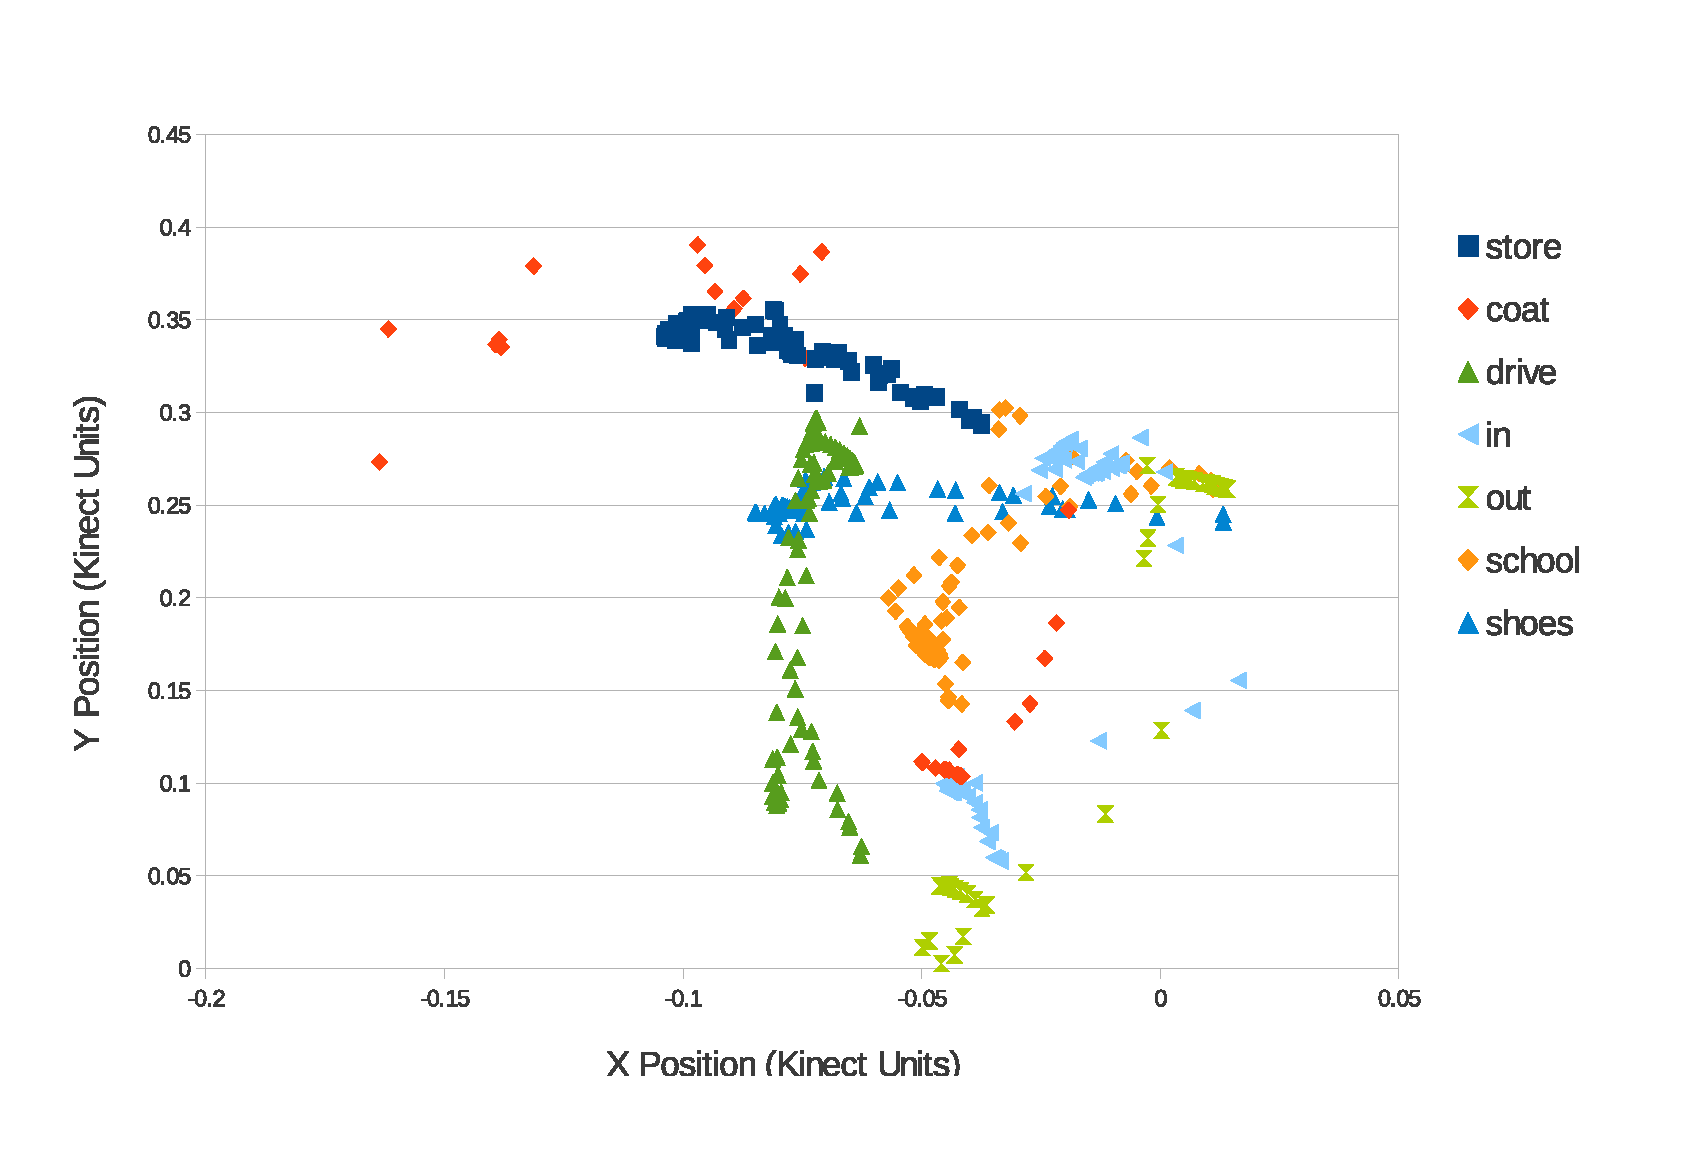
\includegraphics[width=\linewidth]{scatter_plot_left_hand.eps}
\caption{Overlapping Right Hand Positions in ASL Signs}
\label{fig:asl_sign_overlap}
\end{center}
\end{figure}

% BRAD: Thad moved this here because it seemed like a better place than intro
% 7. Present ASL recognition as an example of a complex skill set to identify, as inconsistency and noise are more likely prevalent with human repetitions of actions than precise robotic replay.
Our reasons for using ASL here are several.  First and foremost, ASL requires, at a minimum, a six-dimensional state space representation.  This provides sufficient complexity to prove that our skill representation can be used in environments where brute force and other na\"ive methods would be intractable.  Furthermore, the noise associated with human performance of the ASL symbols is large enough to ensure that our recognition techniques rely on the overall trajectory of the training data, and not merely frame-by-frame matching of exact states over time.  Finally, the ASL gestures chosen overlap significantly avoiding segmentation based on region of the state space that a primitive action occupies. Although there are six dimensions of the state space in total, figure \ref{fig:asl_sign_overlap} displays a representative sampling of the noticeable overlap along two of those dimensions.

Gesture recognition for ASL symbols is not novel.  Our attempt here is not to recognize gestures with an extremely high degree of fidelity.  Although an interesting problem in its own right, several researchers have already made formidable contributions in this arena \cite{HandGestures,HSMMRecognition,POMDPGesture,HoughASL,ASLRealTime,MotionASL}.  What is interesting here is using our system to perform frame-by-frame classification of which gesture is likely being performed, while simultaneously improving the accuracy of an internal policy representing that respective gesture.

\section{Results}
\label{sec:result}

\begin{figure}
\begin{center}
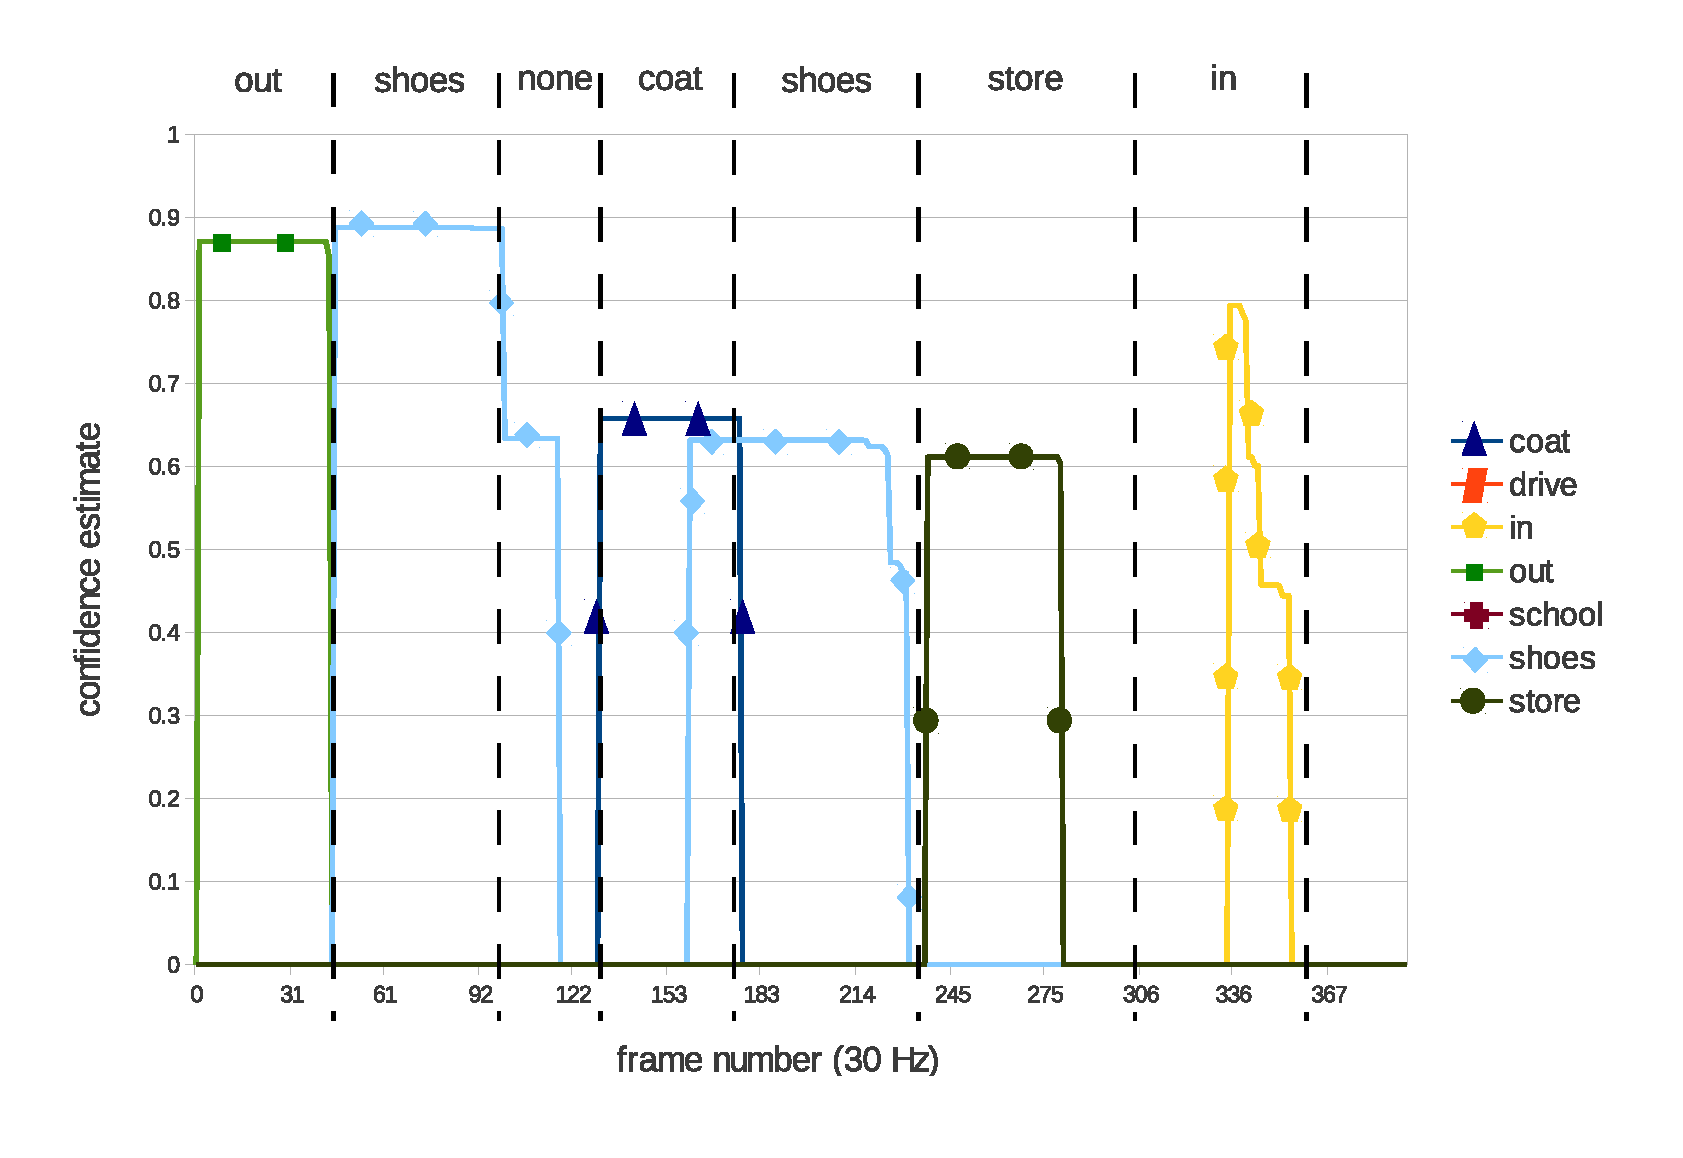
\includegraphics[width=\linewidth]{output_nowaypoints_onetrial.eps}
\caption{Initial Recognition Without Waypointing}
\label{fig:output_nowaypoints_onetrial}
\end{center}
\end{figure}

\begin{figure}
\begin{center}
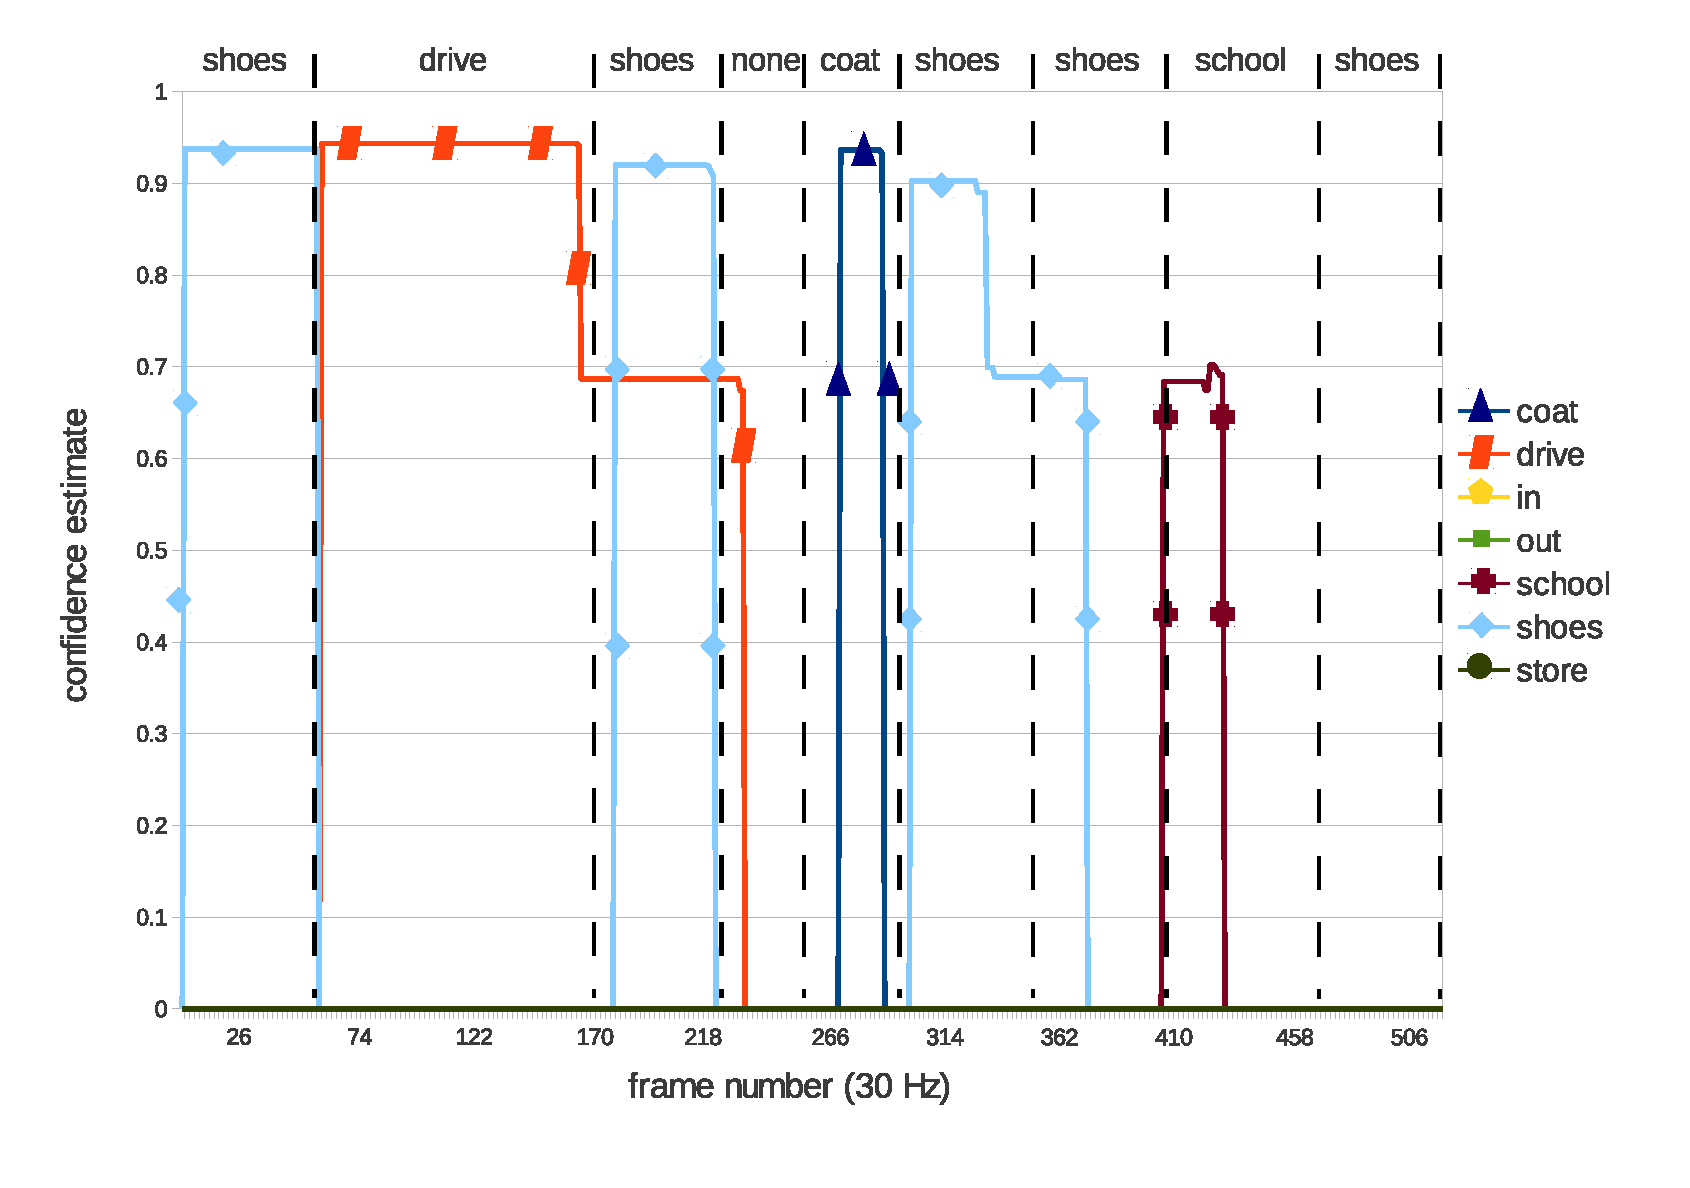
\includegraphics[width=\linewidth]{output_waypoints_repeatedtrials.eps}
\caption{Repeated Recognition Over Time With Waypointing}
\label{fig:output_nowaypoints_repeatedtrials}
\end{center}
\end{figure}

In this section we discuss our experimental results.

\section{Related and Future Work}
\label{sec:future}
It is important to differentiate our contribution from that of
existing research in learning from demonstration.  Much previous research
within reinforcement learning has focused on using examples to
transfer a policy representing some basic skill from teacher to
pupil \cite{JenkinsLFD,LFDSurvey}.  Our algorithm focuses on the use of
\textit{existing knowledge} to generate an approximate decomposition of
complex scene data while simultaneously using our classifications and 
observation to continue to shape actionable policies.

While work partially overlapping our goals has been published previously
\cite{LearningBehaviorFusion}, our work differs substantially in terms of both
our algorithm and the resulting simultaneous benefit to observation
classification and action execution. By categorizing observations into a timeline, a robotic agent may also build a hierarchy by applying subsequence recognition to the algorithm's output. This construction provides an concise, communicable plan for any observed Task. The problem of hierarchy assignment is left for other methods to more fully explore.

Another issue that is left unexplored in this discussion is that of garbage collection.  As we discuss, a crucial part of the algorithm provided is to limit the window of comparison to the length of the recorded primitive plus some epsilon, enabling its feasibility for use as an online algorithm.  However, a separate measure of the ``leanness'' of the algorithm is the amount of memory it consumes.  Currently, every observed state is added to an action's representative MDP, and it is connected to all possible neighboring states via interpolation.  This could easily lead to a ``state space explosion,'' where the primitive skills each contained an enormous amount of unnecessary states in their MDP.  This problem could be solved cursorily by providing a garbage-collector thread that continuously removes states with transitions whose values are below some threshold $\tau$.

Furthermore, it is crucial that this system be deployed in a complex, collaborative, multi-human multi-agent environment.  For example, given a limited set of observation data from a factory floor, a robotic system using our algorithm should have been able to decompose the scene into several agents performing several primitives simultaneously.  Once deployed in the actual factory, the robot should be capable of both performing actions it has learned in cooperation with humans and continue gathering observational data in order to improve its understanding of the task construction and policy execution.


\section{Conclusions}
\label{sec:conclusions}
We have presented herein a method for action recognition that simultaneously leverages an existing representation of primitive skills and improves the accuracy with which those skills can be performed by the observer.  This real-time recognition of learned actions is essential for any co-robot to be able to cooperate effectively in a multi-human multi-robot environment.  

Our system can be easily qualified as an extension to what Ng and Abeel \shortcite{OriginalInverseRL} originally termed ``inverse reinforcement learning''.  By opportunistically incorporating observed data as propagated rewards to the SMDP skill representation, our system converges on a stable learned primitive with fewer trials.  Furthermore, the bonus rewards assigned to those observations that achieve extremely high confidence allows us to treat specific portions of noisy, lossy, and otherwise unreliable observed data as, essentially, expert training.

Other works have offered solutions to many of the challenges standing in the way of mainstreaming collaborative robotics, including automating option scaffolding through demonstration \cite{AutoSkillAcquisition}, acquiring skills utilizing human reward signals in place of \cite{TAMER} or in addition to \cite{TeacherRL} a traditional objective function, and correcting for critical omissions in non-expert demonstrations \cite{PerspectiveTaking}. Simplifying the human trainer/robot student interaction paradigm by shaping human guidance into usable forms is also rapidly advancing \cite{TAMER,Clicker,AdviceTaking,TeacherRL,DemonstrationRL}. These successful results strongly contribute to the widespread use of Q-Learning variants in real robotic systems and, more generally, to the feasibility of real-time human-robot collaboration.

\bibliographystyle{aaai}
\bibliography{report}

\end{document}
